\documentclass[a4paper,14pt]{extarticle}
\usepackage[utf8]{inputenc}
\usepackage[russian]{babel}
\usepackage{graphicx}
\usepackage[top=0.8in, bottom=0.8in, left=0.8in, right=0.8in]
{geometry}
\usepackage{pgfplots}
\usepackage{amsmath}
\usepackage{setspace}
\usepackage{titlesec}
\usepackage{float}
\usepackage{chngcntr}
\usepackage{pgfplots}
\usepackage{amsfonts}
\usepackage{pgfplotstable}
\usepackage{multirow}
\usepackage{karnaugh-map}
\usepackage{tikz,xcolor}
\usepackage{indentfirst} % Красная строка
\usepackage{listings}
\usepackage{amssymb}
\usepackage{xcolor}
\usepackage{hyperref}

\definecolor{linkcolor}{HTML}{0000FF} % цвет ссылок
\definecolor{urlcolor}{HTML}{FF00FF} % цвет гиперссылок

\hypersetup{pdfstartview=FitH, linkcolor=linkcolor,urlcolor=urlcolor, colorlinks=true}


\titleformat{\section}[hang]
  {\bfseries}
  {}
  {0em}
  {\hspace{-0.4pt}\large \thesection\hspace{0.6em}}
  
  
\titleformat{\subsection}[hang]
  {\bfseries}
  {}
  {0em}
  {\hspace{-0.4pt}\large \thesubsection\hspace{0.6em}}

%\linespread{1.3} % полуторный интервал
%\renewcommand{\rmdefault}{ftm} % Times New Roman

\newcommand{\nx}{\overline{x}}
\newcommand{\p}{0.31}
\newcommand{\scale}{1.4}

\counterwithin{figure}{section}
\counterwithin{equation}{section}
\counterwithin{table}{section}

\begin{document}
\begin{titlepage}
\centering
Санкт-Петербургский политехнический университет Петра Великого \\
\vspace{0.15cm}
Кафедра компьютерных систем и программных технологий \\
\vspace{6.5cm}

{\centering \textbf{Отчёт по лабораторной работе} \\ 
\vspace{0.15cm}
\textbf{Дисциплина}: Телекоммуникационные технологии \\
\vspace{0.15cm}
\textbf{Тема}: Аналоговая, частотная и фазовая модуляция.} \\


\vspace{6.5cm}

\begin{table}[H]
\begin{tabular}{p{\textwidth}@{}r}
{Выполнил студент гр. 33501/2} \hfill {Вахаев И.Н.} \\
{Преподаватель} \hfill {Богач Н.В.} \\
\end{tabular}
\end{table}
\vfill

{\centering Санкт-Петербург \\ 
\vspace{0.15cm}
\today}
\end{titlepage}

\tableofcontents

\newpage

\section{Цель работы}

Изучение амплитудной частотной и фазовой модуляции/демодуляции сигнала.

\section{Постановка задачи}

\begin{enumerate}
\item Сгенерировать однотональный сигнал низкой частоты.

\item Выполнить амплитудную модуляцию (АМ) сигнала по закону
$$ u(t) = (1 + MU_m cos(\Omega t)) cos(\omega_0 t + \phi_0)$$
для различных значений глубины модуляции M. Используйте встроенную функцию MatLab $ammod$.

Выполнить фазовую модуляцию/демодуляцию сигнала по закону 
$$ u(t) = U_m cos(\Omega t + ks(t)$$
используя встроенную функцию MatLab $pmmod$, $pmdemod$

\item Получить спектр модулированного сигнала.

\item Выполнить модуляцию с подавлением несущей.
$$ u(t) = MU_m cos(\Omega t) cos(\omega_0 t + \phi_0)$$
получить спектр.
\item Выполнить однополосную модуляцию:
$$\displaystyle u(t) = U_m cos(\Omega t) cos(\omega_0 t + \phi_0) + \frac{U_m}{2} \sum^N_{n=1}M_n(cos(\omega_0 + \Omega_n) t + \phi_0 + \Phi_n)$$
положив n=1.

\item Выполнить частотную модуляцию/демодуляцию по закону
$$\displaystyle u(t) = U_m cos(\omega_0 t + k \int_0^t s(t)dt + \phi_0)$$
используя встроенные функции MatLab $fmmod$, $fmdemod$.

\item Выполнить синхронное детектирование и получить исходный
однополосный сигнал.

\item Рассчитать КПД модуляции.
$$\displaystyle \eta_{AM} = \frac{U^2_m M^2/4}{P_U} = \frac{M^2}{M^2 + 2}$$
\end{enumerate}

\section{Теоретический раздел}

Модуляция — процесс изменения одного или нескольких параметров модулируемого несущего сигнала при помощи модулирующего сигнала.

Передаваемая информация заложена в модулирующем сигнале, а роль переносчика информации выполняет высокочастотное колебание, называемое несущим (модулируемым). Модуляция, таким образом, представляет собой процесс «посадки» информационного колебания на заведомо известную несущую с целью получения нового модулированного сигнала.

В результате модуляции спектр низкочастотного управляющего сигнала переносится в область высоких частот. Это позволяет при организации вещания настроить функционирование всех приёмо-передающих устройств на разных частотах с тем, чтобы они «не мешали» друг другу.

В качестве несущего могут быть использованы колебания различной формы (прямоугольные, треугольные и т. д.), однако чаще всего применяются гармонические колебания. В зависимости от того, какой из параметров несущего колебания изменяется, различают вид модуляции (амплитудная, частотная, фазовая и др.). Модуляция дискретным сигналом называется цифровой модуляцией или манипуляцией.

Различают три основных вида модуляции – амплитудную, частотную и фазовую.

\subsection{Амплитудная модуляции}

Амплитудная модуляция (AM) — наиболее распространенный тип модуляции. В системе с AM амплитуда несущей изменяется в соответствии с изменением сигнала или информации. В отсутствие сигнала амплитуда несущей имеет постоянный уровень. При модуляции синусоидальным сигналом амплитуда несущей увеличивается или уменьшается относительно своего немодулированного уровня по синусоидальному закону в соответствии с нарастанием или спаданием модулирующего сигнала. Чем больше амплитуда модулирующего сигнала, тем сильнее изменяется амплитуда несущей. Амплитудно-модулированная несущая имеет огибающую, в точности повторяющую форму модулирующего сигнала, и при демодуляции именно эта огибающая выделяется как полезный сигнал.

\subsection{Частотная модуляции}

Частотной модуляцией называется вид аналоговой модуляции, при которой, частота несущей изменяется по закону модулирующего низкочастотного сигнала. Амплитуда при этом остается постоянной.

Наибольшее отклонение частоты от среднего значения, называется девиацией.
В идеальном варианте, девиация должна быть прямо пропорционально амплитуде модулирующего колебания.

Спектр при частотной модуляции состоит из несущей и симметрично отстающей от нее вправо и влево гармоник боковых полос, на частоту кратную частоте модулирующего колебания.
Данный спектр представляет гармоническое колебание. В случае реальной модуляции, спектр имеет более сложные очертания.
Различают широкополосную и узкополосную ЧМ модуляцию.
В широкополосной — спектр частот, значительно превосходит частоту модулирующего сигнала. Применяется в ЧМ радиовещании.
В радиостанциях применяют в основном узкополосную ЧМ модуляцию, требующую более точной настройки приемника и соответственно более защищенную от помех.

Спектр узкополосной ЧМ напоминает амплитудную модуляцию, но если учесть фазу боковых полос, то окажется, что эти волны имеют постоянную амплитуду и переменную частоту, а не постоянную частоту и переменную амплитуду (AM). При широкополосной ЧМ амплитуда несущей может быть очень малой, что обусловливает высокую эффективность ЧМ; это значит, что большая часть передаваемой энергии содержится в боковых частотах, несущих информацию.

Основные преимущества ЧМ, перед АМ — энергоэффективность и помехоустойчивость.

\subsection{Фазовая модуляции}

Фазовая модуляция - процесс изменения фазы несущего сигнала в соответствии с мгновенными значениями модулирующего сигнала.

По характеристикам фазовая модуляция близка к частотной модуляции. В случае синусоидального модулирующего (информационного) сигнала, результаты частотной и фазовой модуляции совпадают. В аналоговой технике фазовая модуляция используется реже, чем частотная, поскольку требует более сложного преобразования при приеме.

Максимальное отклонение фазы модулированного сигнала относительно среднего значения называется девиацией фазы, задается в угловых единицах (градус, радиан).

Достоинствами фазовой модуляции являются: высокая помехоустойчивость, более эффективное использование мощности передатчика.

Недостатками фазовой модуляции являются: большая ширина спектра, сравнительная трудность получения модулированных сигналов и их детектирование.

\newpage


\section{Ход работы}

\subsection{Амплитудная модуляция}

В среде Simulink была создана схема, необходимая для проведения амплитудной модуляции (Рисунок \ref{0}). В дальнейшем для частотной и фазовой модуляций схема будет изменена, а параметры синусоидального сигнала (Рисунок \ref{1}) оставим с действующими настройками. 

\begin{figure}[H]
\center{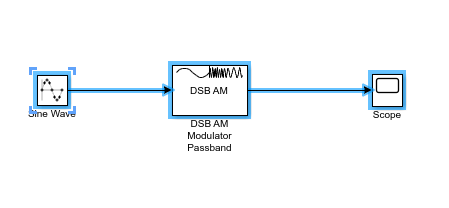
\includegraphics[width=1\linewidth]{screen/0}}
\caption{Схема для проведения амплитудной модуляции}
\label{0}
\end{figure}

\begin{figure}[H]
\center{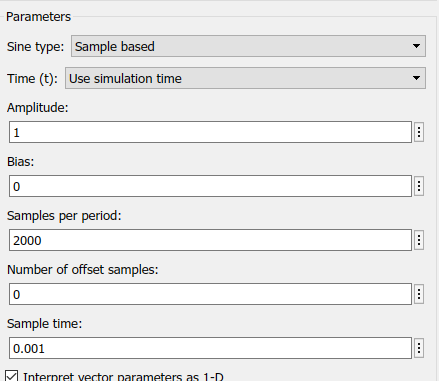
\includegraphics[width=1\linewidth]{screen/1}}
\caption{Параметры синусоидального сигнала}
\label{1}
\end{figure}

На рисунке \ref{2} представлены параметры амплитудного модулятора.

\begin{figure}[H]
\center{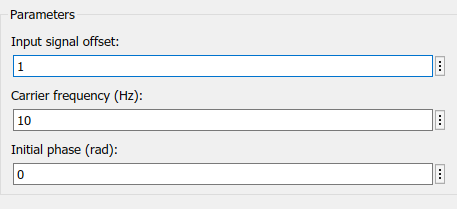
\includegraphics[width=1\linewidth]{screen/2}}
\caption{Параметры амплитудного модулятора}
\label{2}
\end{figure}

Получили амплитудную модуляцию сигнала (Рисунок \ref{3}

\begin{figure}[H]
\center{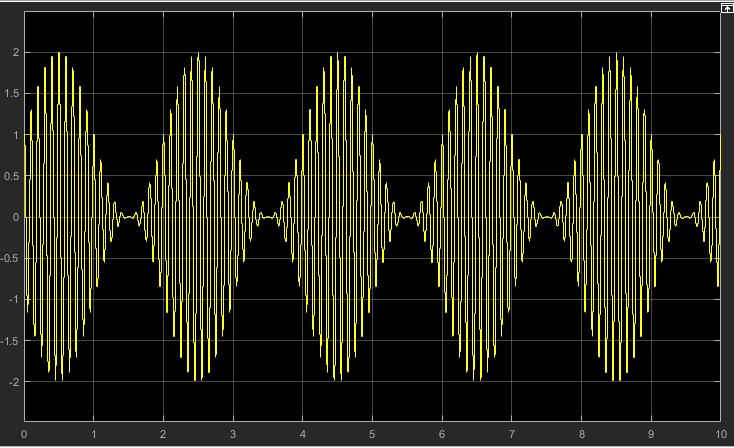
\includegraphics[width=1\linewidth]{screen/3}}
\caption{Амплитудная модуляция}
\label{3}
\end{figure}

Для получения информационного сигнала вкупе с исходным сигналом необходимо модифицировать схему. Представим её на рисунке \ref{4}.

\begin{figure}[H]
\center{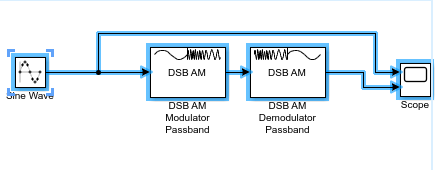
\includegraphics[width=1\linewidth]{screen/4}}
\caption{Схема для амплитудной демодуляции}
\label{4}
\end{figure}

Был добавлен амплитудный демодулятор. В конечном итоге получили результирующий сигнал после демодуляции вкупе с исходным сигналом (Рисунок \ref{5}).

\begin{figure}[H]
\center{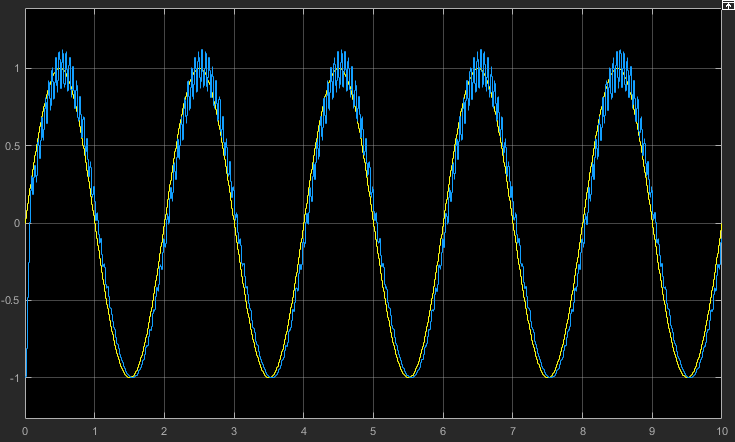
\includegraphics[width=1\linewidth]{screen/5}}
\caption{Исходный и демодулированный амплитудный сигнал}
\label{5}
\end{figure}

Добавим Spectrum Analyzer для получения спектра моделированного сигнала. Модифицированная схема представлена на рисунке \ref{6}.

\begin{figure}[H]
\center{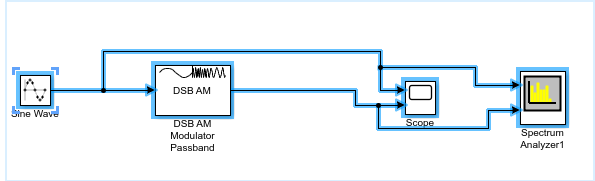
\includegraphics[width=1\linewidth]{screen/6}}
\caption{Схема для получения спектра моделированного сигнала}
\label{6}
\end{figure}

Был получен спектр(в Watts) модулированного сигнала такого вида(Рисунок \ref{7}):

\begin{figure}[H]
\center{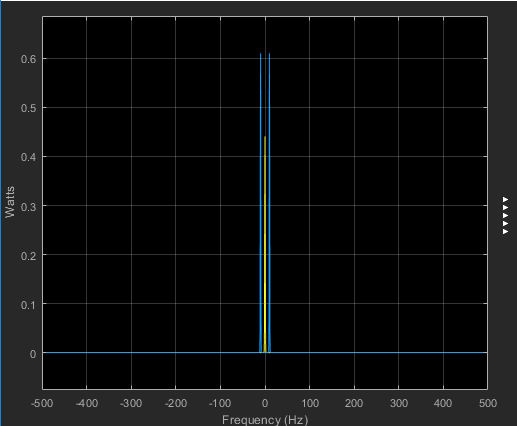
\includegraphics[width=1\linewidth]{screen/7}}
\caption{Спектр моделированного сигнала и исходного сигнала}
\label{7}
\end{figure}

Также получили спектр в dBm (Рисунок \ref{8}):

\begin{figure}[H]
\center{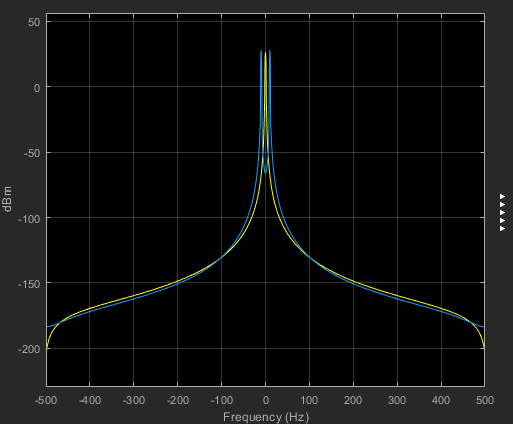
\includegraphics[width=1\linewidth]{screen/8}}
\caption{Спектр моделированного сигнала и исходного сигнала}
\label{8}
\end{figure}

Модифицируем схему для получения спектра демодулированного сигнала вкупе с исходным(Рисунок \ref{9}):

\begin{figure}[H]
\center{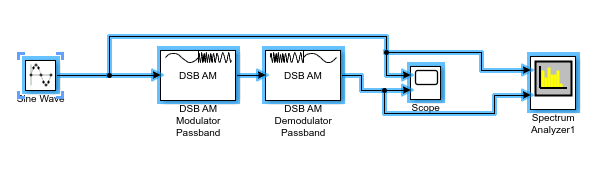
\includegraphics[width=1\linewidth]{screen/9}}
\caption{Схема для получения спектра демодулированного сигнала}
\label{9}
\end{figure}

Был получен спектр(в Watts) демодулированного сигнала такого вида(Рисунок \ref{10}):

\begin{figure}[H]
\center{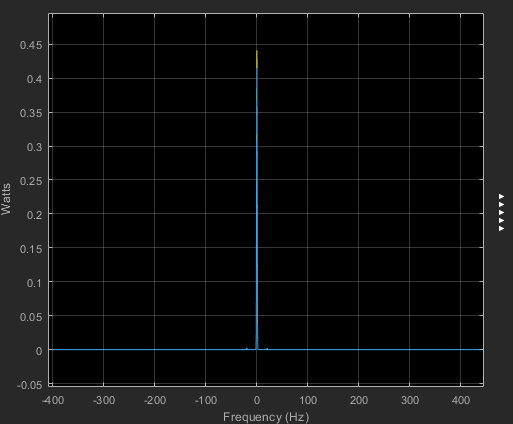
\includegraphics[width=1\linewidth]{screen/10}}
\caption{Спектр демоделированного сигнала и исходного сигнала}
\label{10}
\end{figure}

Также получили спектр в dBm (Рисунок \ref{11}):

\begin{figure}[H]
\center{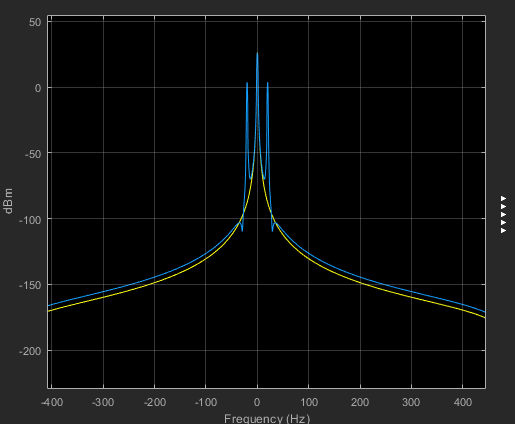
\includegraphics[width=1\linewidth]{screen/11}}
\caption{Спектр демоделированного сигнала и исходного сигнала}
\label{11}
\end{figure}

\subsection{Частотная модуляция}

Модифицируем схему для исследования амплитудной модуляции для исследования частотной модуляции. Модифицированная схема представлена на рисунке \ref{12}.

\begin{figure}[H]
\center{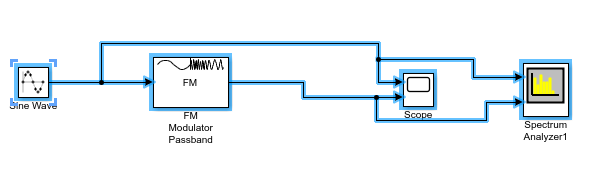
\includegraphics[width=1\linewidth]{screen/12}}
\caption{Схема для исследования частотной модуляции}
\label{12}
\end{figure}

Параметры частотного модулятора представлены на рисунке \ref{13}.

\begin{figure}[H]
\center{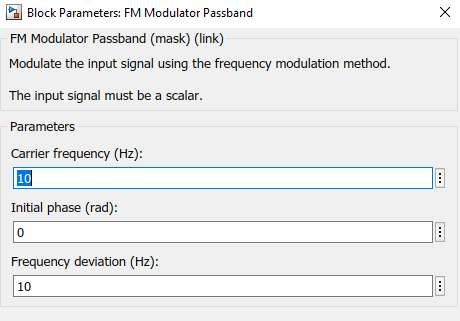
\includegraphics[width=1\linewidth]{screen/13}}
\caption{Параметры частотного модулятора}
\label{13}
\end{figure}

Частотная модуляция исходного сигнала выглядит следующим образом(Рисунок \ref{14}):

\begin{figure}[H]
\center{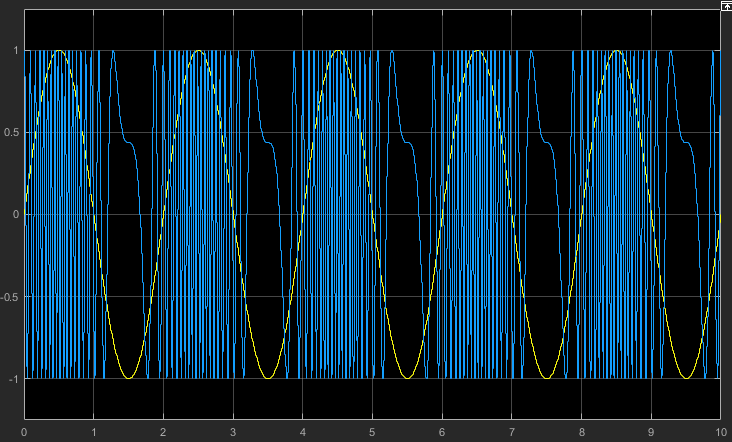
\includegraphics[width=1\linewidth]{screen/14}}
\caption{Частотная модуляция исходного сигнала}
\label{14}
\end{figure}

Были получены спектры модулированного сигнала в Watts(Рисунок \ref{15}) и в dBm(Рисунок \ref{16}).

\begin{figure}[H]
\center{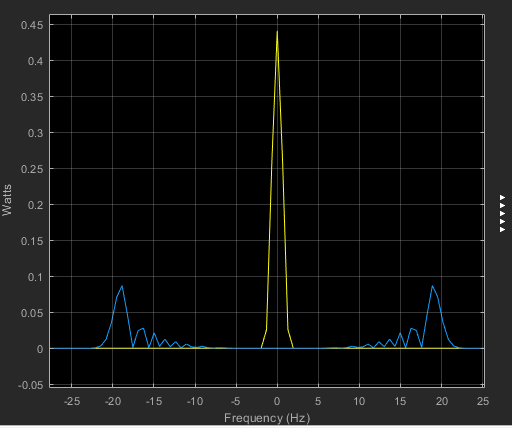
\includegraphics[width=1\linewidth]{screen/15}}
\caption{Спектры исходного и модулированного сигнала(Watts)}
\label{15}
\end{figure}

\begin{figure}[H]
\center{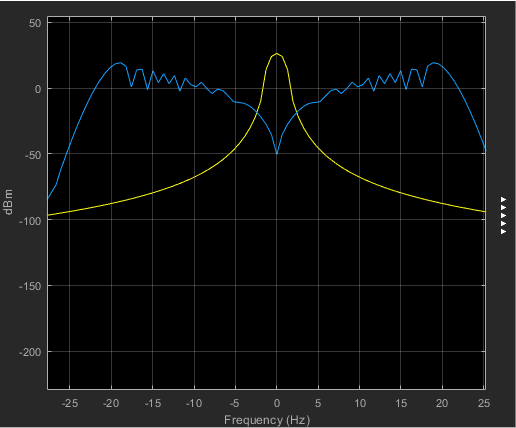
\includegraphics[width=1\linewidth]{screen/16}}
\caption{Спектры исходного и модулированного сигнала(dBm)}
\label{16}
\end{figure}

Модифицируем схему для демодуляции сигнала(Рисунок \ref{17}).

\begin{figure}[H]
\center{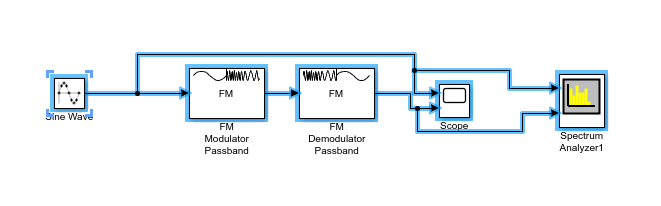
\includegraphics[width=1\linewidth]{screen/17}}
\caption{Схема для демодуляции сигнала}
\label{17}
\end{figure}

Параметры демодулятора представлены на рисунке \ref{18}.

\begin{figure}[H]
\center{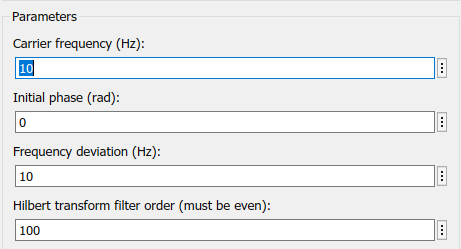
\includegraphics[width=1\linewidth]{screen/18}}
\caption{Схема для демодуляции сигнала}
\label{18}
\end{figure}

Результат демодуляции сигнала выглядит следующим образом(Рисунок \ref{19}):

\begin{figure}[H]
\center{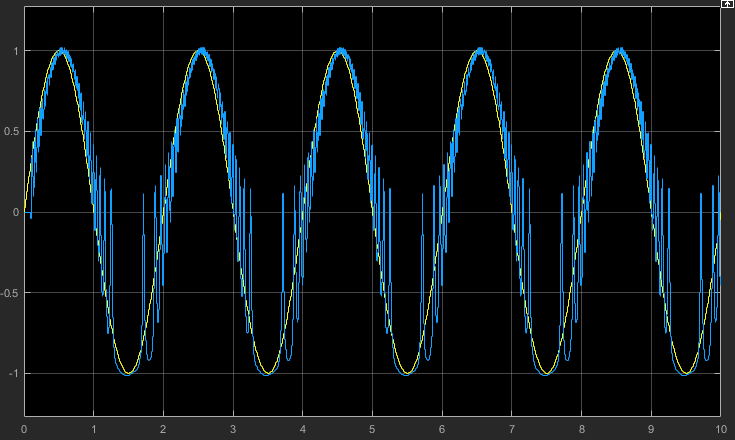
\includegraphics[width=1\linewidth]{screen/19}}
\caption{Демодуляция сигнала}
\label{19}
\end{figure}

Спектры демодулированного сигнала в Watts(Рисунок \ref{20}) и в dBm(Рисунок \ref{21}):

\begin{figure}[H]
\center{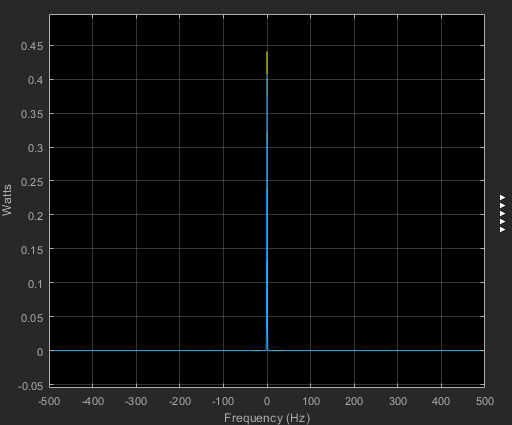
\includegraphics[width=1\linewidth]{screen/20}}
\caption{Спектры исходного и демодулированного сигнала(Watts)}
\label{20}
\end{figure}

\begin{figure}[H]
\center{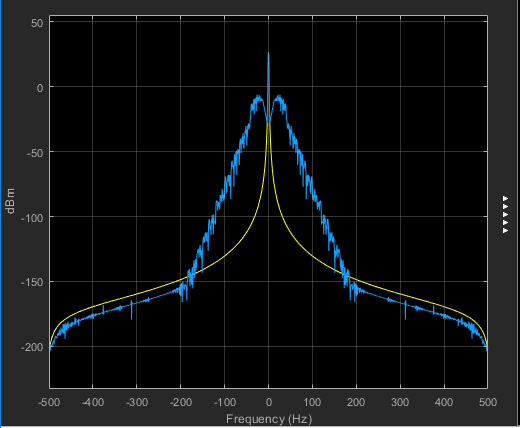
\includegraphics[width=1\linewidth]{screen/21}}
\caption{Спектры исходного и демодулированного сигнала(dBm)}
\label{21}
\end{figure}


\subsection{Фазовая модуляция}

Модифицируем схему используемую для исследования частотной модуляции для исследования фазовой модуляции. Модифицированная схема представлена на рисунке \ref{22}.

\begin{figure}[H]
\center{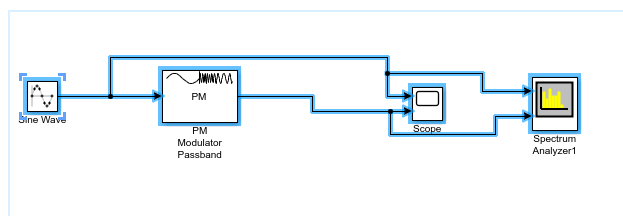
\includegraphics[width=1\linewidth]{screen/22}}
\caption{Схема для фазовой модуляции)}
\label{22}
\end{figure}

Параметры фазового модулятора представлены на рисунке \ref{23}.

\begin{figure}[H]
\center{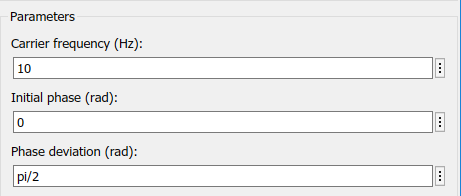
\includegraphics[width=1\linewidth]{screen/23}}
\caption{Параметры фазового модулятора)}
\label{23}
\end{figure}

На рисунке \ref{24} представлен результат фазовой модуляции сигнала.

\begin{figure}[H]
\center{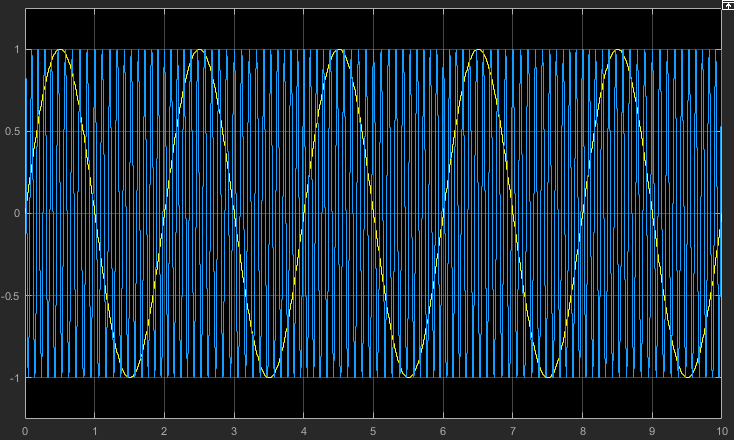
\includegraphics[width=1\linewidth]{screen/24}}
\caption{Фазовая модуляция сигнала)}
\label{24}
\end{figure}

Спектры модулированного сигнала в Watts(Рисунок \ref{25}) и в dBm(Рисунок \ref{26}):

\begin{figure}[H]
\center{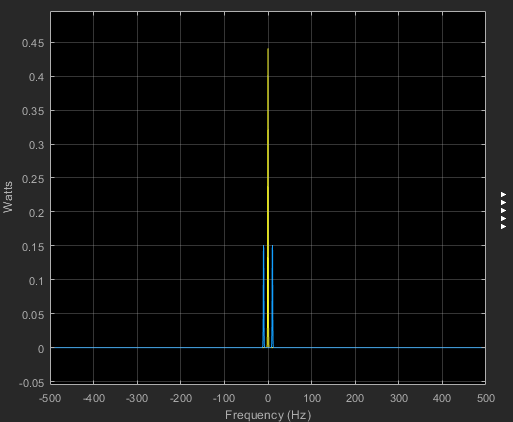
\includegraphics[width=1\linewidth]{screen/25}}
\caption{Спектры исходного и модулированного сигнала(Watts)}
\label{25}
\end{figure}

\begin{figure}[H]
\center{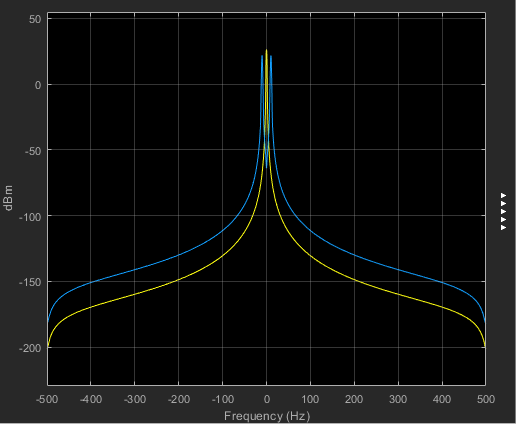
\includegraphics[width=1\linewidth]{screen/26}}
\caption{Спектры исходного и модулированного сигнала(dBm)}
\label{26}
\end{figure}

Модифицируем схему, представленную на рисунке \ref{22}. Добавив фазовый демодулятор получили следующую схему(Рисунок  \ref{27}):

\begin{figure}[H]
\center{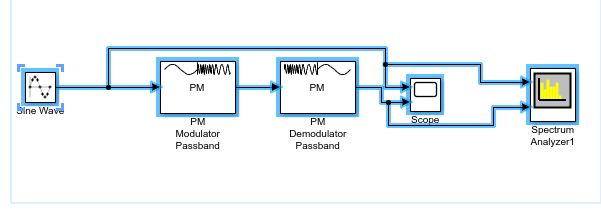
\includegraphics[width=1\linewidth]{screen/27}}
\caption{Схема для демодуляции сигнала}
\label{27}
\end{figure}

Параметры фазового демодулятора представлены на рисунке \ref{28}.

\begin{figure}[H]
\center{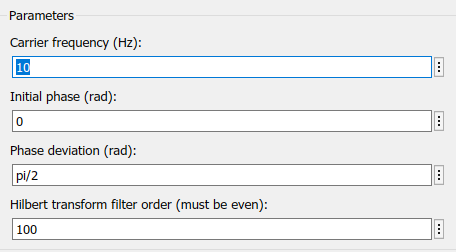
\includegraphics[width=1\linewidth]{screen/28}}
\caption{Параметры фазового демодулятора}
\label{28}
\end{figure}

Результат демодуляции сигнала выглядит следующим образом(Рисунок \ref{29}):

\begin{figure}[H]
\center{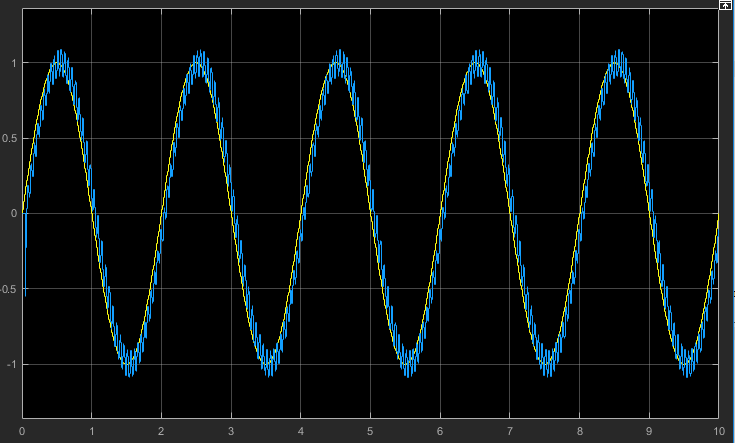
\includegraphics[width=1\linewidth]{screen/29}}
\caption{Демодуляция сигнала}
\label{29}
\end{figure}

Спектры демодулированного сигнала в Watts(Рисунок \ref{30}) и в dBm(Рисунок \ref{31}):

\begin{figure}[H]
\center{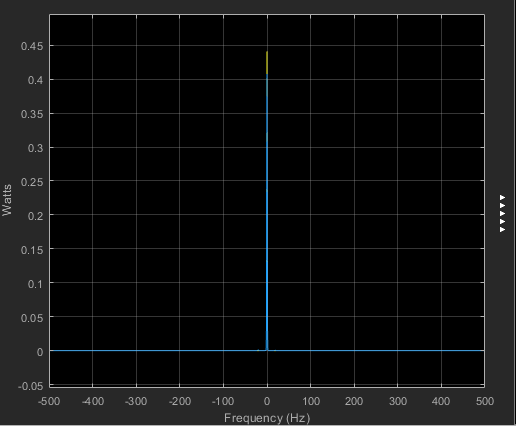
\includegraphics[width=1\linewidth]{screen/30}}
\caption{Спектры исходного и демодулированного сигнала(Watts)}
\label{30}
\end{figure}

\begin{figure}[H]
\center{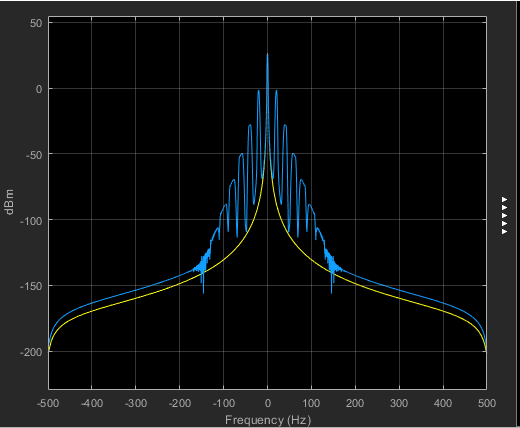
\includegraphics[width=1\linewidth]{screen/31}}
\caption{Спектры исходного и демодулированного сигнала(dBm)}
\label{31}
\end{figure}


\section{Выводы}

В данной лабораторной работе были исследованы методы аналоговой, частотной и фазовой модуляции/демодуляции.

При амплитудной модуляции мы изменяем амплитуду сигнала, оставляя неизменными частоту и фазу. Применяется такая модуляция редко, так как имеет низкий КПД равный 33 процентам. Помехонеустойчивость возникает вследствие узкой полосы модулируемого сигнала. Амплитудную модуляцию используют в основном в средне- и низкочастотных интервалах электромагнитного спектра.
Частотная модуляция является видом аналоговой модуляции, при котором информационный сигнал управляет частотой несущего колебания с постоянной амплитудой. Она применяется для высококачественной передачи звукового сигнала в радиовещании, для звукового сопровождения телевизионных программ и т.д. Такая модуляция характеризуется высокой помехоустойчивостью, однако для ее применения следует использовать высокочастотный диапазон.
Фазовая модуляция является видом модуляции, при которой фаза несущего колебания изменяется прямо пропорционально информационному сигналу. По характеристикам данная модуляция близка к частотной модуляции. Фазовая модуляция активно используется для формирования помехозащищенной связи в микроволновом диапазоне.


\end{document}